\section{Query Processing}

\subsection{Khái niệm Query Processing}
Query Processing là quá trình hệ quản trị cơ sở dữ liệu tiếp nhận yêu cầu truy vấn, phân tích cú pháp, tối ưu kế hoạch thực thi và trả về kết quả cho người dùng. Chất lượng của cơ chế xử lý truy vấn ảnh hưởng trực tiếp đến độ trễ, throughput và khả năng biểu diễn các nghiệp vụ phức tạp.

\subsection{Cách tiếp cận của MySQL và Redis}
\begin{table}[H]
\centering
\caption{So sánh cách xử lý truy vấn giữa MySQL và Redis}
\label{tab:query-processing-overview}
\begin{tabular}{|p{3.2cm}|p{5.2cm}|p{5.2cm}|}
\hline
\textbf{Tiêu chí} & \textbf{MySQL} & \textbf{Redis} \\ \hline
Ngôn ngữ truy vấn & SQL khai báo, giàu khả năng biểu diễn & Lệnh đơn giản, kết hợp Lua script để xử lý logic \\ \hline
Optimizer & Có query optimizer, execution plan, cost-based optimization & Không có optimizer cho truy vấn phức tạp; ứng dụng phải tự quyết định cách truy xuất \\ \hline
JOIN / GROUP BY & Hỗ trợ native, tối ưu nội bộ & Không hỗ trợ native; phải mô phỏng bằng nhiều lệnh hoặc Lua script \\ \hline
Aggregate / Sort / Limit & Hỗ trợ trực tiếp bằng SQL & Phải duyệt dữ liệu, gom nhóm và sắp xếp thủ công \\ \hline
Độ linh hoạt & Phù hợp truy vấn phân tích và nghiệp vụ nhiều quan hệ & Phù hợp truy cập trực tiếp theo key hoặc tập dữ liệu đã chuẩn bị sẵn \\ \hline
\end{tabular}
\end{table}

\subsubsection{MySQL}
MySQL tiếp cận theo mô hình truy vấn khai báo: người dùng mô tả \textit{cần lấy dữ liệu gì}, còn hệ quản trị tự quyết định \textit{lấy bằng cách nào}. Với bộ tối ưu truy vấn, MySQL có thể:
\begin{itemize}
    \item chọn index phù hợp cho điều kiện lọc;
    \item tối ưu thứ tự JOIN giữa nhiều bảng;
    \item thực hiện GROUP BY, ORDER BY, LIMIT và subquery trực tiếp;
    \item khi cần phân tích sâu, có thể dùng \texttt{EXPLAIN} ngoài phần liệt kê mã nguồn truy vấn chính.
\end{itemize}

\subsubsection{Redis}
Redis không phải là hệ quản trị hướng truy vấn quan hệ. Thế mạnh của Redis là truy cập dữ liệu theo key với độ trễ rất thấp. Khi cần truy vấn phức tạp hơn, lập trình viên phải:
\begin{itemize}
    \item thiết kế key và set index ngay từ đầu;
    \item tự kết hợp nhiều lệnh \texttt{HGET}, \texttt{SMEMBERS}, \texttt{ZRANGE}, \texttt{SINTER};
    \item dùng Lua script để gom nhiều bước thành một thao tác phía server;
    \item chấp nhận rằng aggregate, sort và filtering phức tạp thường phải scan nhiều key.
\end{itemize}

\subsection{Môi trường và dữ liệu thử nghiệm}
Phần thực nghiệm sử dụng bộ dữ liệu BikeStores đã được import vào cả hai hệ:
\begin{itemize}
    \item \textbf{MySQL:} dữ liệu nằm trong hai schema \texttt{production} và \texttt{sales}.
    \item \textbf{Redis:} dữ liệu được ánh xạ dưới dạng \texttt{Hash} cho thực thể và \texttt{Set} cho các tập chỉ mục.
\end{itemize}

\begin{figure}[H]
\centering
\begin{minipage}{0.48\textwidth}
\centering
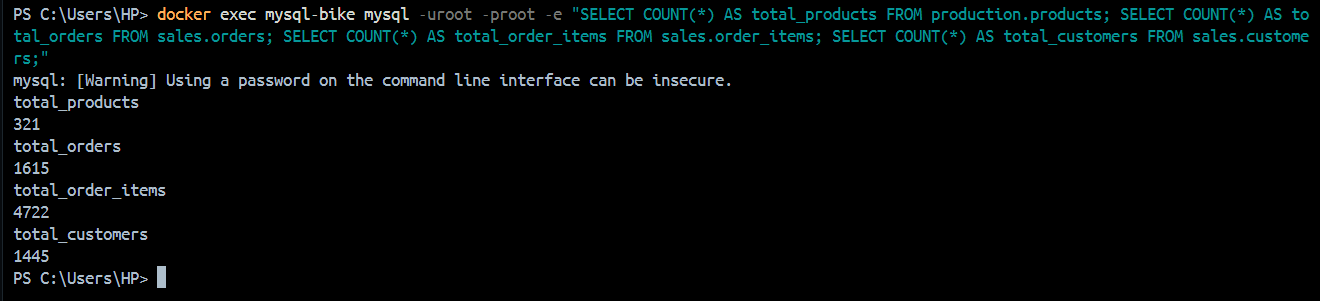
\includegraphics[width=\linewidth]{figures/Trung/count_record-mysql.png}
\caption{Số bản ghi kiểm tra phía MySQL.}
\label{fig:mysql-count}
\end{minipage}
\hfill
\begin{minipage}{0.48\textwidth}
\centering
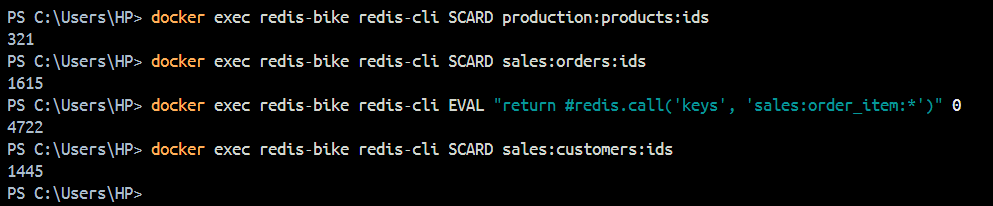
\includegraphics[width=\linewidth]{figures/Trung/count_record-redis.png}
\caption{Số key kiểm tra phía Redis.}
\label{fig:redis-count}
\end{minipage}
\end{figure}

\begin{table}[H]
\centering
\caption{Các bảng và key chính được sử dụng trong phần Query Processing}
\label{tab:query-dataset}
\small
\setlength{\tabcolsep}{4pt}
\begin{tabular}{|p{2.75cm}|p{5.15cm}|p{7.15cm}|}
\hline
\textbf{Nghiệp vụ} & \textbf{MySQL} & \textbf{Redis} \\ \hline
Sản phẩm theo danh mục &
\texttt{production.products} &
\begin{minipage}[t]{\linewidth}\raggedright
\texttt{production:product:\{id\}}\\
\texttt{production:products:category:}
\texttt{\{category\_id\}}
\end{minipage} \\ \hline
Chi tiết đơn hàng &
\begin{minipage}[t]{\linewidth}\raggedright
\texttt{sales.orders}\\
\texttt{sales.order\_items}\\
\texttt{production.products}
\end{minipage} &
\begin{minipage}[t]{\linewidth}\raggedright
\texttt{sales:order:\{id\}}\\
\texttt{sales:order\_item:\{order\_id\}:}
\texttt{\{item\_id\}}
\end{minipage} \\ \hline
Doanh thu theo cửa hàng &
\begin{minipage}[t]{\linewidth}\raggedright
\texttt{sales.stores}\\
\texttt{sales.orders}\\
\texttt{sales.order\_items}
\end{minipage} &
\begin{minipage}[t]{\linewidth}\raggedright
\texttt{sales:orders:store:\{store\_id\}}\\
\texttt{Hash sales:order\_item:\{order\_id\}:}
\texttt{\{item\_id\}}
\end{minipage} \\ \hline
Khách hàng chưa phát sinh đơn &
\begin{minipage}[t]{\linewidth}\raggedright
\texttt{sales.customers}\\
\texttt{sales.orders}
\end{minipage} &
\begin{minipage}[t]{\linewidth}\raggedright
\texttt{sales:customers:ids}\\
\texttt{sales:orders:customer:}
\texttt{\{customer\_id\}}
\end{minipage} \\ \hline
\end{tabular}
\normalsize
\end{table}

\subsection{Thực nghiệm truy vấn}
\subsubsection{Truy vấn đơn giản trên một bảng}\par

\textbf{Mục tiêu:} lấy tất cả sản phẩm thuộc category ``Mountain Bikes'' (\texttt{category\_id = 6}) và sắp xếp theo giá giảm dần.

\textbf{MySQL}
\begin{lstlisting}[language=SQL, basicstyle=\ttfamily\small, breaklines=true, frame=single]
SELECT product_id, product_name, list_price
FROM production.products
WHERE category_id = 6
ORDER BY list_price DESC;
\end{lstlisting}

\textbf{Redis}
\begin{lstlisting}[language={}, basicstyle=\ttfamily\small, breaklines=true, frame=single]
redis-cli EVAL "
local pids = redis.call('SMEMBERS', 'production:products:category:6')
local result = {}
for _, pid in ipairs(pids) do
    local p = redis.call('HGETALL', 'production:product:' .. pid)
    local info = {}
    for i = 1, #p, 2 do info[p[i]] = p[i+1] end
    table.insert(result, {tonumber(info.list_price),
        pid .. ' | ' .. info.product_name .. ' | $' .. info.list_price})
end
table.sort(result, function(a, b) return a[1] > b[1] end)
local output = {}
for _, r in ipairs(result) do table.insert(output, r[2]) end
return output
" 0
\end{lstlisting}

\textbf{Nhận xét:} Đây là loại truy vấn Redis xử lý khá tốt vì đã có set index theo danh mục. Tuy nhiên Redis vẫn phải tự tải từng hash và tự sắp xếp trong Lua, trong khi MySQL biểu diễn cùng nghiệp vụ ngắn gọn hơn bằng một câu SQL duy nhất.

\begin{figure}[H]
\centering
\begin{minipage}{0.48\textwidth}
\centering
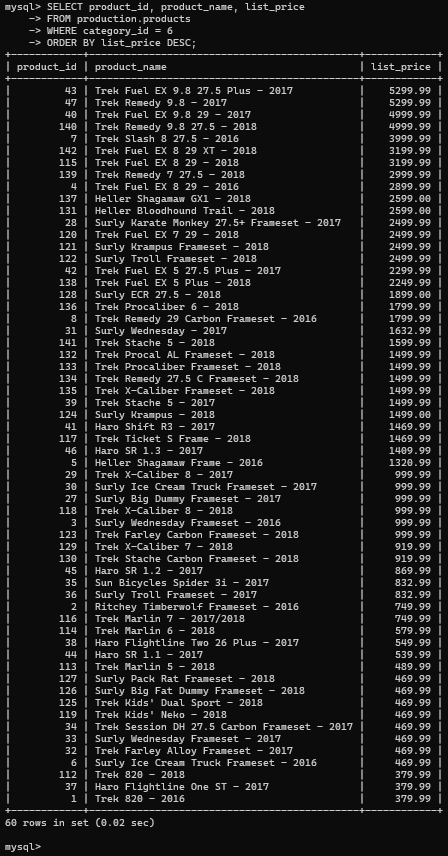
\includegraphics[width=\linewidth]{figures/Trung/q1-mysql.png}
\caption{Kết quả Q1 trên MySQL.}
\label{fig:q1-mysql}
\end{minipage}
\hfill
\begin{minipage}{0.48\textwidth}
\centering
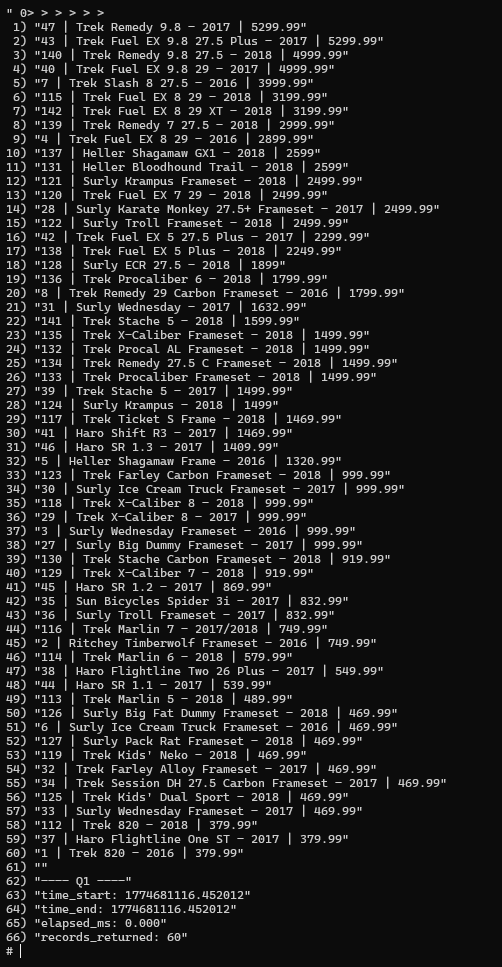
\includegraphics[width=\linewidth]{figures/Trung/q1-redis.png}
\caption{Kết quả Q1 trên Redis (Lua \texttt{EVAL}).}
\label{fig:q1-redis}
\end{minipage}
\end{figure}

\subsubsection{Truy vấn JOIN nhiều bảng}

\textbf{Mục tiêu:} lấy chi tiết đơn hàng số 1, bao gồm tên sản phẩm, số lượng, giá và tổng tiền từng dòng.

\textbf{MySQL}
\begin{lstlisting}[language=SQL, basicstyle=\ttfamily\small, breaklines=true, frame=single]
SELECT o.order_id, o.order_date, p.product_name,
       oi.quantity, oi.list_price, oi.discount,
       (oi.quantity * oi.list_price * (1 - oi.discount)) AS line_total
FROM sales.orders o
JOIN sales.order_items oi ON o.order_id = oi.order_id
JOIN production.products p ON oi.product_id = p.product_id
WHERE o.order_id = 1;
\end{lstlisting}

\textbf{Redis}
\begin{lstlisting}[language={}, basicstyle=\ttfamily\small, breaklines=true, frame=single]
redis-cli EVAL "
local item_ids = redis.call('SMEMBERS', 'sales:order_items:order:1')
local result = {}
for _, iid in ipairs(item_ids) do
    local item = redis.call('HGETALL', 'sales:order_item:1:' .. iid)
    local info = {}
    for i = 1, #item, 2 do info[item[i]] = item[i+1] end
    local pname = redis.call('HGET', 'production:product:' .. info.product_id, 'product_name')
    local total = tonumber(info.quantity) * tonumber(info.list_price) * (1 - tonumber(info.discount))
    table.insert(result, pname .. ' | qty:' .. info.quantity .. ' | $' .. info.list_price ..
        ' | disc:' .. info.discount .. ' | total: ' .. string.format('%.4f', total))
end
return result
" 0
\end{lstlisting}

\textbf{Nhận xét:} MySQL thể hiện lợi thế rất rõ ở JOIN vì quan hệ giữa các bảng đã được mô hình hóa sẵn bằng khóa ngoại. Trong Redis, JOIN không tồn tại theo nghĩa native mà phải ghép nhiều key bằng tay, nên truy vấn dài hơn và khó bảo trì hơn.

\begin{figure}[H]
\centering
\begin{minipage}{0.48\textwidth}
\centering
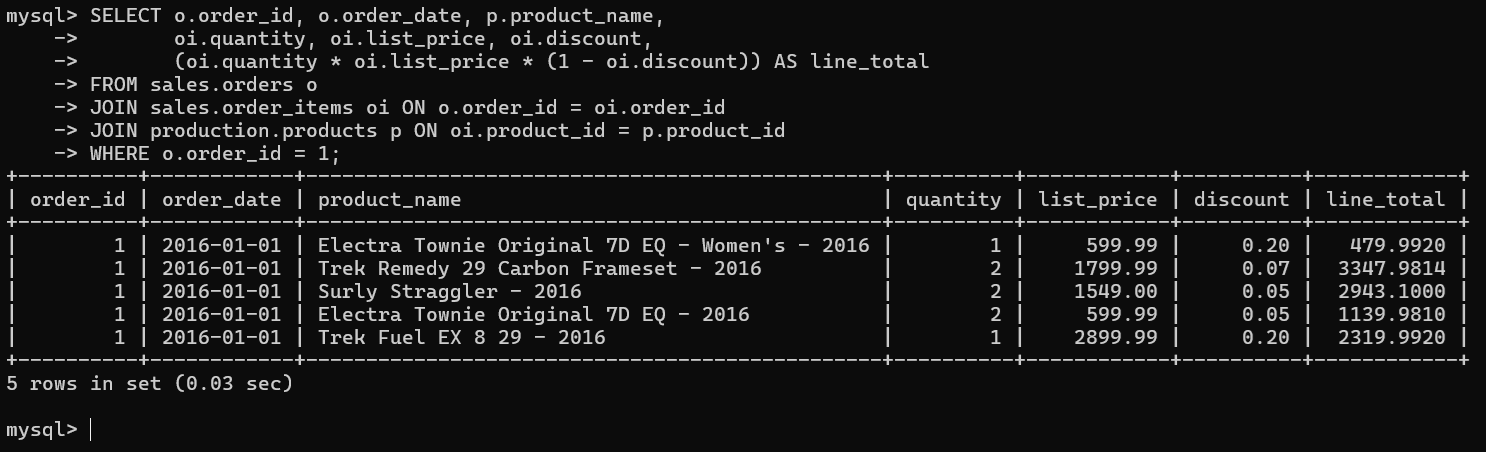
\includegraphics[width=\linewidth]{figures/Trung/q2-mysql.png}
\caption{Kết quả Q2 trên MySQL.}
\label{fig:q2-mysql}
\end{minipage}
\hfill
\begin{minipage}{0.48\textwidth}
\centering
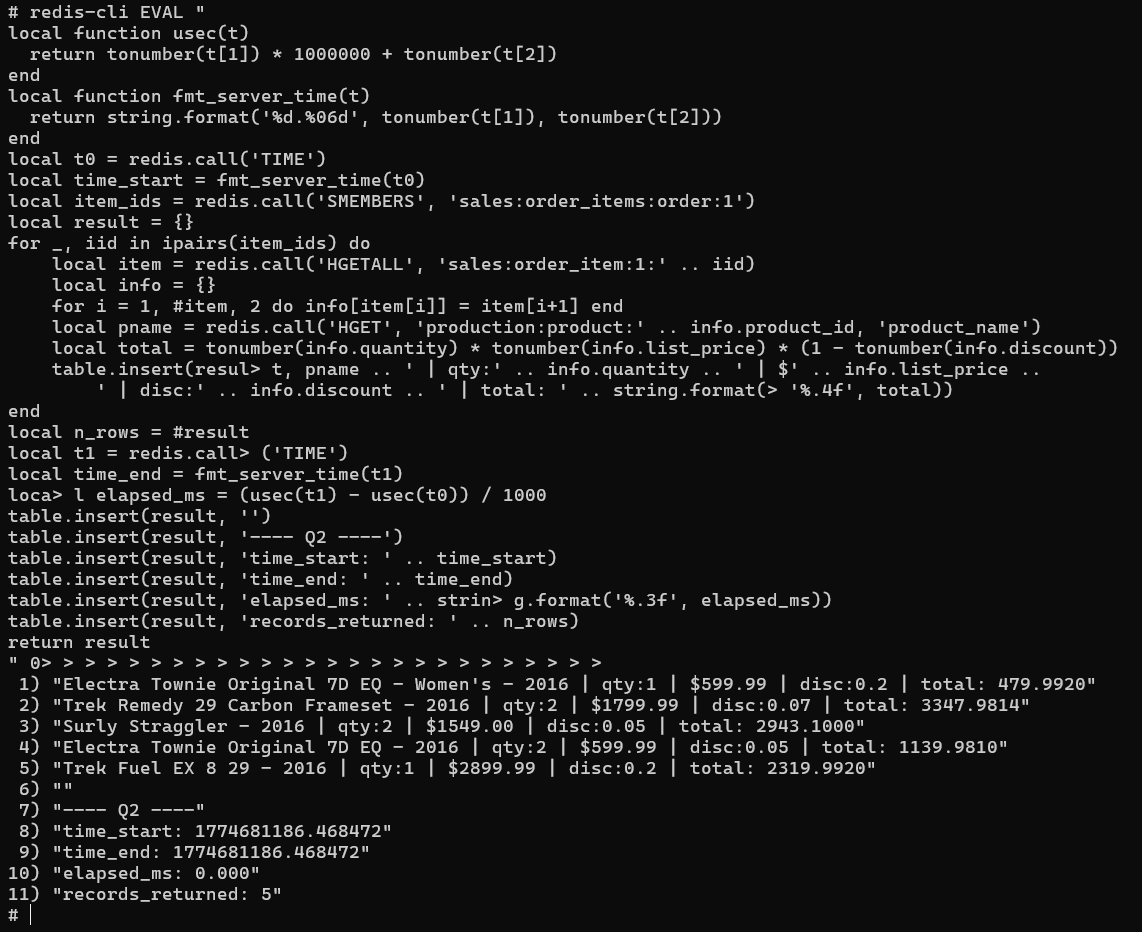
\includegraphics[width=\linewidth]{figures/Trung/q2-redis.png}
\caption{Kết quả Q2 trên Redis.}
\label{fig:q2-redis}
\end{minipage}
\end{figure}

\subsubsection{Truy vấn gom nhóm và tính tổng}

\textbf{Mục tiêu:} tính tổng doanh thu theo từng cửa hàng.

\textbf{MySQL}
\begin{lstlisting}[language=SQL, basicstyle=\ttfamily\small, breaklines=true, frame=single]
SELECT s.store_name,
       COUNT(DISTINCT o.order_id) AS total_orders,
       SUM(oi.quantity * oi.list_price * (1 - oi.discount)) AS revenue
FROM sales.stores s
JOIN sales.orders o ON s.store_id = o.store_id
JOIN sales.order_items oi ON o.order_id = oi.order_id
GROUP BY s.store_name
ORDER BY revenue DESC;
\end{lstlisting}

\textbf{Redis}
\begin{lstlisting}[language={}, basicstyle=\ttfamily\small, breaklines=true, frame=single]
redis-cli EVAL "
local stores = redis.call('SMEMBERS', 'sales:stores:ids')
local rows = {}
for _, sid in ipairs(stores) do
    local name = redis.call('HGET', 'sales:store:' .. sid, 'store_name')
    local oids = redis.call('SMEMBERS', 'sales:orders:store:' .. sid)
    local revenue = 0
    for _, oid in ipairs(oids) do
        local iids = redis.call('SMEMBERS', 'sales:order_items:order:' .. oid)
        for _, iid in ipairs(iids) do
            local key = 'sales:order_item:' .. oid .. ':' .. iid
            local q = tonumber(redis.call('HGET', key, 'quantity'))
            local p = tonumber(redis.call('HGET', key, 'list_price'))
            local d = tonumber(redis.call('HGET', key, 'discount'))
            revenue = revenue + (q * p * (1 - d))
        end
    end
    table.insert(rows, {revenue, #oids, name})
end
table.sort(rows, function(a, b) return a[1] > b[1] end)
local result = {}
for _, r in ipairs(rows) do
    table.insert(result, r[3] .. ' | Orders: ' .. r[2] ..
        ' | Revenue: ' .. string.format('%.4f', r[1]))
end
return result
" 0
\end{lstlisting}

\textbf{Nhận xét:} Đây là nhóm truy vấn Redis bất lợi nhất vì phải quét qua rất nhiều key rồi tự cộng dồn thủ công. MySQL xử lý tốt hơn nhờ engine tối ưu cho aggregate, grouping và join theo quan hệ.

\begin{figure}[H]
\centering
\begin{minipage}{0.48\textwidth}
\centering
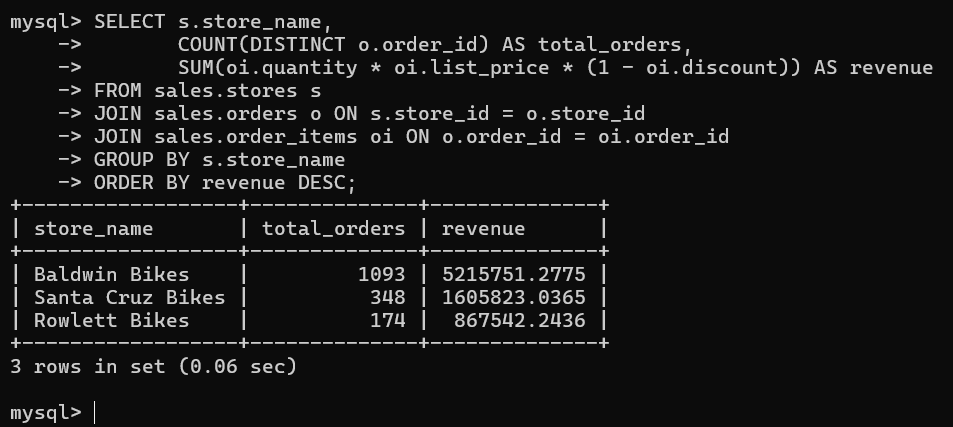
\includegraphics[width=\linewidth]{figures/Trung/q3-mysql.png}
\caption{Kết quả Q3 trên MySQL.}
\label{fig:q3-mysql}
\end{minipage}
\hfill
\begin{minipage}{0.48\textwidth}
\centering
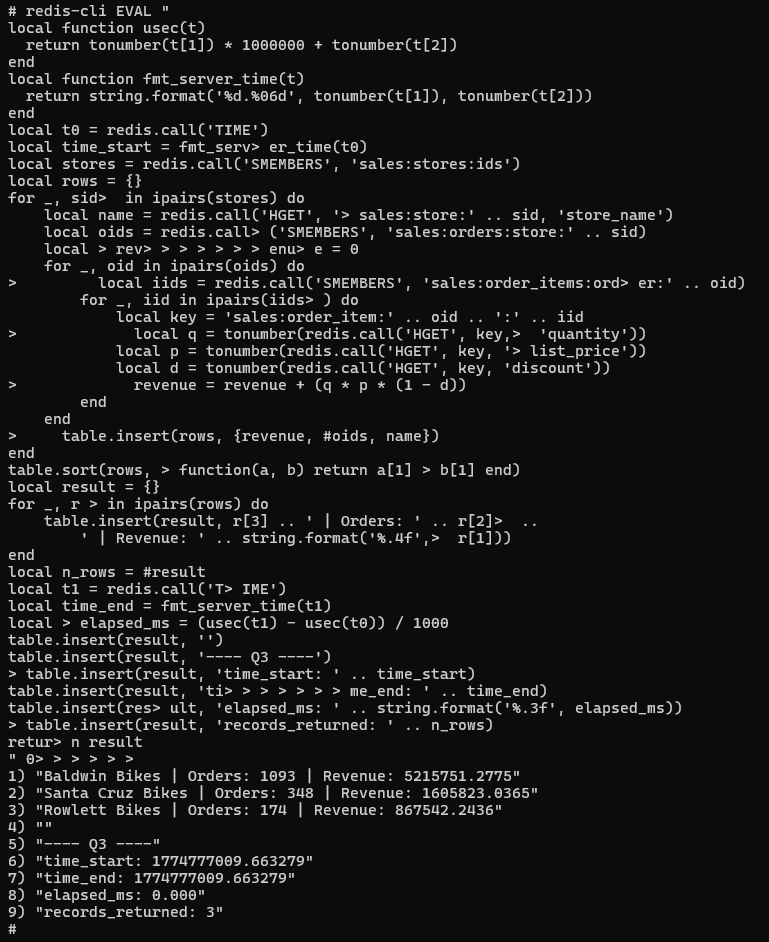
\includegraphics[width=\linewidth]{figures/Trung/q3-redis.png}
\caption{Kết quả Q3 trên Redis.}
\label{fig:q3-redis}
\end{minipage}
\end{figure}

\begin{figure}[H]
\centering
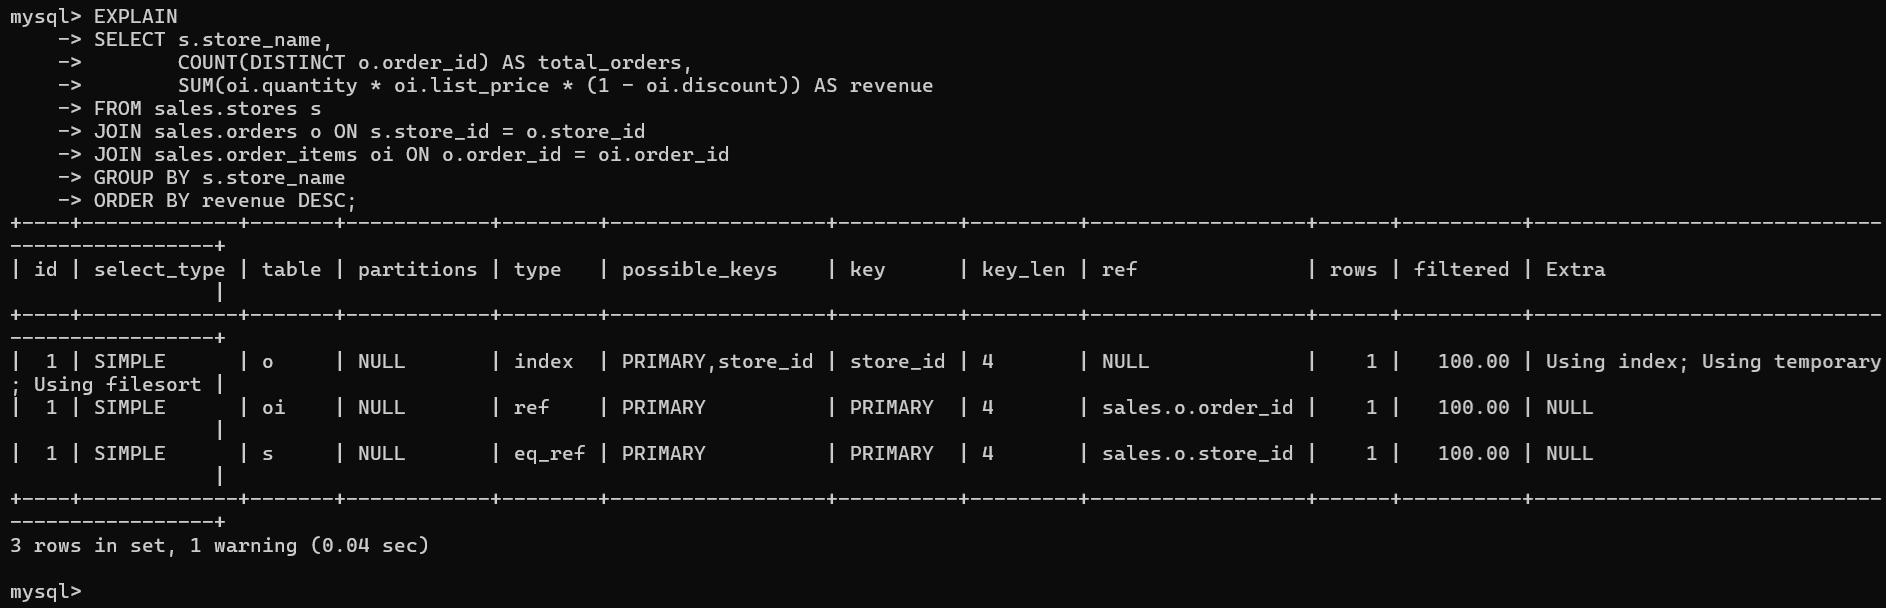
\includegraphics[width=0.92\textwidth]{figures/Trung/q3-explain-mysql.png}
\caption{Execution plan (\texttt{EXPLAIN}) cho Q3 trên MySQL — minh họa cách optimizer ước lượng chi phí.}
\label{fig:q3-explain}
\end{figure}

\subsubsection{Truy vấn Top-N}

\textbf{Mục tiêu:} tìm 5 sản phẩm bán chạy nhất theo tổng số lượng bán ra.

\textbf{MySQL}
\begin{lstlisting}[language=SQL, basicstyle=\ttfamily\small, breaklines=true, frame=single]
SELECT p.product_id, p.product_name, SUM(oi.quantity) AS total_sold
FROM sales.order_items oi
JOIN production.products p ON oi.product_id = p.product_id
GROUP BY p.product_id
ORDER BY total_sold DESC
LIMIT 5;
\end{lstlisting}
\textit{Ghi chú:} BikeStores có nhiều \texttt{product\_id} trùng \texttt{product\_name}; chỉ \texttt{GROUP BY p.product\_id} (không gom theo tên) để khớp Redis.

\textbf{Redis}
\begin{lstlisting}[language={}, basicstyle=\ttfamily\small, breaklines=true, frame=single]
redis-cli EVAL "
local pids = redis.call('SMEMBERS', 'production:products:ids')
local sales = {}
for _, pid in ipairs(pids) do sales[pid] = 0 end
local oids = redis.call('SMEMBERS', 'sales:orders:ids')
for _, oid in ipairs(oids) do
    local iids = redis.call('SMEMBERS', 'sales:order_items:order:' .. oid)
    for _, iid in ipairs(iids) do
        local key = 'sales:order_item:' .. oid .. ':' .. iid
        local pid = redis.call('HGET', key, 'product_id')
        local qty = tonumber(redis.call('HGET', key, 'quantity'))
        if sales[pid] then sales[pid] = sales[pid] + qty end
    end
end
local sorted = {}
for pid, qty in pairs(sales) do
    if qty > 0 then
        local name = redis.call('HGET', 'production:product:' .. pid, 'product_name')
        table.insert(sorted, {qty, name, pid})
    end
end
table.sort(sorted, function(a, b) return a[1] > b[1] end)
local result = {}
for i = 1, math.min(5, #sorted) do
    table.insert(result, '#' .. i .. ' | id ' .. sorted[i][3] .. ' | ' .. sorted[i][2] .. ' | Sold: ' .. sorted[i][1])
end
return result
" 0
\end{lstlisting}

\textbf{Nhận xét:} Top-N là dạng truy vấn tiêu biểu cho sự khác biệt giữa hai hệ. Với MySQL, đây là truy vấn tổng hợp tiêu chuẩn. Với Redis, nếu không thiết kế sẵn sorted set hoặc materialized leaderboard thì phải quét toàn bộ dữ liệu rồi sắp xếp thủ công, gây tốn CPU và thời gian.

\begin{figure}[H]
\centering
\begin{minipage}{0.48\textwidth}
\centering
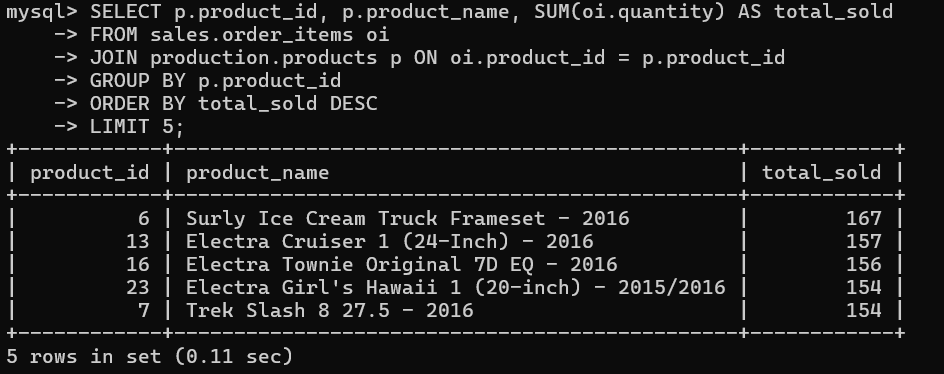
\includegraphics[width=\linewidth]{figures/Trung/q4-mysql.png}
\caption{Kết quả Q4 trên MySQL.}
\label{fig:q4-mysql}
\end{minipage}
\hfill
\begin{minipage}{0.48\textwidth}
\centering
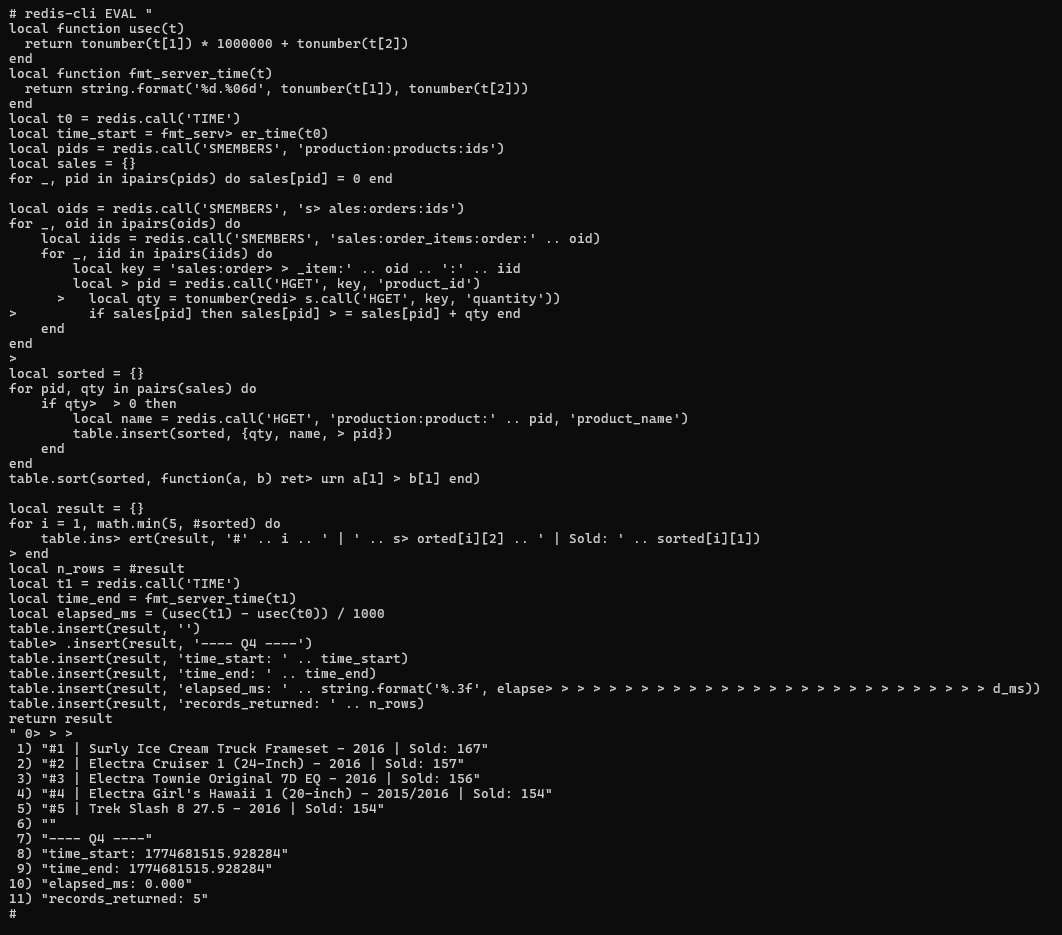
\includegraphics[width=\linewidth]{figures/Trung/q4-redis.png}
\caption{Kết quả Q4 trên Redis.}
\label{fig:q4-redis}
\end{minipage}
\end{figure}

\begin{figure}[H]
\centering
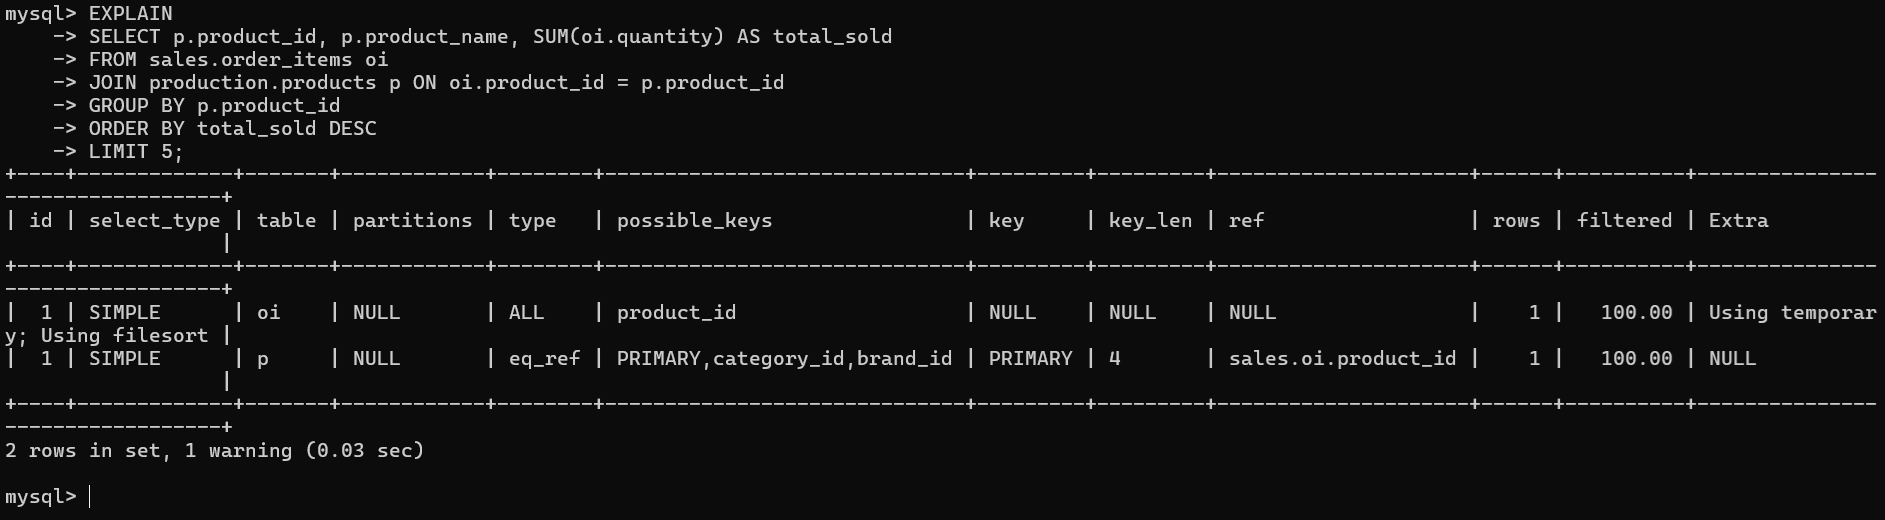
\includegraphics[width=0.92\textwidth]{figures/Trung/q4-explain-mysql.png}
\caption{Execution plan (\texttt{EXPLAIN}) cho Q4 trên MySQL.}
\label{fig:q4-explain}
\end{figure}

\subsubsection{Truy vấn lồng nhau / anti-join}

\textbf{Mục tiêu:} tìm các khách hàng chưa từng phát sinh đơn hàng.

\textbf{MySQL}
\begin{lstlisting}[language=SQL, basicstyle=\ttfamily\small, breaklines=true, frame=single]
SELECT c.customer_id, c.first_name, c.last_name
FROM sales.customers c
WHERE c.customer_id NOT IN (
    SELECT DISTINCT customer_id
    FROM sales.orders
    WHERE customer_id IS NOT NULL
);
\end{lstlisting}

\textbf{Redis}
\begin{lstlisting}[language={}, basicstyle=\ttfamily\small, breaklines=true, frame=single]
redis-cli EVAL "
local cids = redis.call('SMEMBERS', 'sales:customers:ids')
local result = {}
for _, cid in ipairs(cids) do
    local oids = redis.call('SMEMBERS', 'sales:orders:customer:' .. cid)
    if #oids == 0 then
        local fname = redis.call('HGET', 'sales:customer:' .. cid, 'first_name')
        local lname = redis.call('HGET', 'sales:customer:' .. cid, 'last_name')
        table.insert(result, cid .. ' | ' .. fname .. ' ' .. lname)
    end
end
return result
" 0
\end{lstlisting}

\textbf{Nhận xét:} MySQL hỗ trợ tự nhiên cho dạng anti-join hoặc subquery. Redis chỉ có thể đạt cùng kết quả nếu ta thiết kế sẵn set đơn hàng theo từng khách hàng; nếu thiếu cấu trúc đó thì chi phí truy vấn sẽ tăng rất mạnh. Với bộ BikeStores mặc định, danh sách khách chưa có đơn có thể rỗng.

\begin{figure}[H]
\centering
\begin{minipage}{0.48\textwidth}
\centering
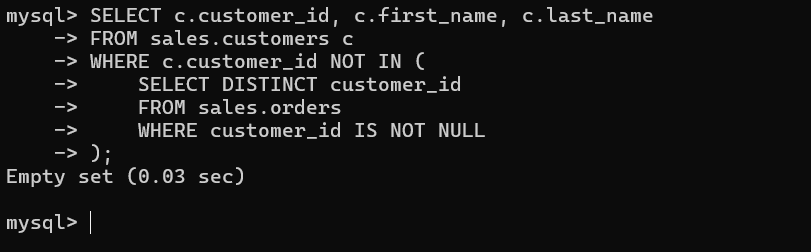
\includegraphics[width=\linewidth]{figures/Trung/q5-mysql.png}
\caption{Kết quả Q5 trên MySQL.}
\label{fig:q5-mysql}
\end{minipage}
\hfill
\begin{minipage}{0.48\textwidth}
\centering
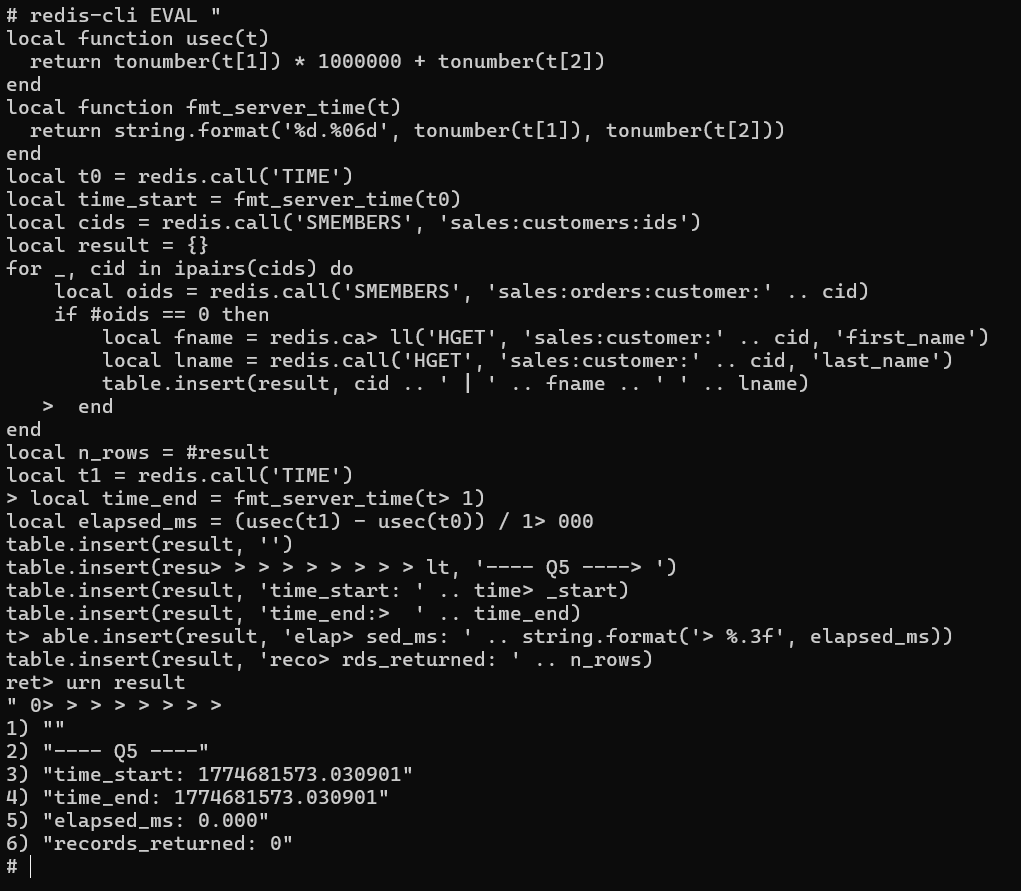
\includegraphics[width=\linewidth]{figures/Trung/q5-redis.png}
\caption{Kết quả Q5 trên Redis.}
\label{fig:q5-redis}
\end{minipage}
\end{figure}

\begin{figure}[H]
\centering
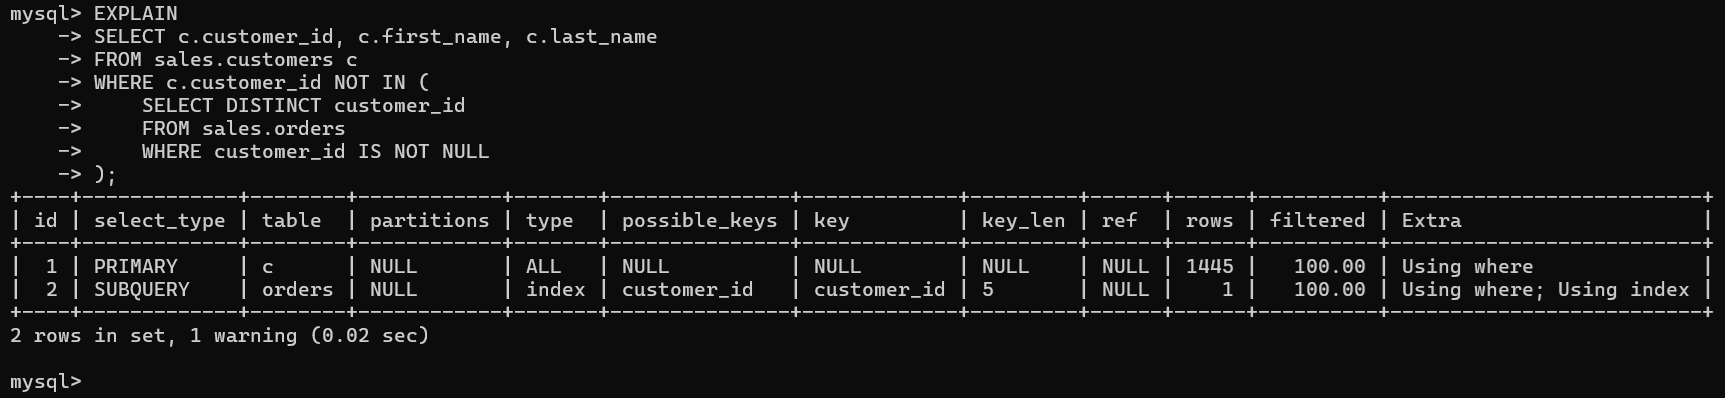
\includegraphics[width=0.92\textwidth]{figures/Trung/q5-explain-mysql.png}
\caption{Execution plan (\texttt{EXPLAIN}) cho Q5 trên MySQL.}
\label{fig:q5-explain}
\end{figure}

\subsection{Phân tích sâu hơn về khả năng biểu diễn truy vấn}
\subsubsection{Độ phức tạp triển khai}
\begin{itemize}
    \item Với MySQL, phần lớn truy vấn nghiệp vụ chỉ cần viết SQL đúng logic.
    \item Với Redis, hiệu quả phụ thuộc mạnh vào thiết kế key, set index và việc chấp nhận duplicate data để phục vụ truy vấn.
    \item Điều này cho thấy Redis thường dịch chuyển chi phí từ ``lúc truy vấn'' sang ``lúc thiết kế mô hình dữ liệu''.
\end{itemize}

\subsubsection{Khả năng mở rộng truy vấn}
\begin{itemize}
    \item Khi yêu cầu nghiệp vụ thay đổi, MySQL thường chỉ cần sửa câu SQL hoặc thêm index.
    \item Trong Redis, thay đổi nghiệp vụ có thể buộc phải tạo thêm key pattern, thêm set index hoặc đồng bộ lại dữ liệu.
    \item Vì vậy Redis phù hợp hơn với các truy vấn truy cập nhanh, cấu trúc đã biết trước và lặp lại nhiều lần.
\end{itemize}

\subsection{Tổng hợp ưu và nhược điểm}
\begin{table}[H]
\centering
\caption{Tổng hợp ưu và nhược điểm của MySQL và Redis trong Query Processing}
\label{tab:query-summary}
\begin{tabular}{|p{2.5cm}|p{5cm}|p{5cm}|}
\hline
 & \textbf{MySQL} & \textbf{Redis} \\ \hline
\textbf{Ưu điểm} & Hỗ trợ SQL đầy đủ, JOIN, GROUP BY, ORDER BY, subquery và optimizer mạnh. & Truy cập theo key cực nhanh, latency thấp, rất hiệu quả cho truy vấn đơn giản hoặc dữ liệu đã được tiền xử lý. \\ \hline
\textbf{Nhược điểm} & Không nhanh bằng Redis trong các truy cập key-value cực đơn giản. & Thiếu ngôn ngữ truy vấn quan hệ, khó bảo trì khi số lượng truy vấn nghiệp vụ tăng, aggregate và sorting phức tạp thường chậm. \\ \hline
\end{tabular}
\end{table}

\subsection{Kết luận}
Từ các truy vấn đã phân tích, có thể thấy MySQL phù hợp hơn cho các hệ thống nghiệp vụ cần truy vấn linh hoạt, nhiều bảng quan hệ, tổng hợp dữ liệu và thống kê. Redis phù hợp hơn khi yêu cầu chính là truy xuất cực nhanh theo key, đọc dữ liệu đã được chuẩn bị trước hoặc dùng làm lớp cache cho các kết quả truy vấn nặng.

Nếu hệ thống cần cả hai mục tiêu, hướng triển khai hợp lý là:
\begin{itemize}
    \item dùng MySQL làm nguồn dữ liệu chính cho các truy vấn nghiệp vụ và báo cáo;
    \item dùng Redis để cache kết quả các truy vấn phổ biến hoặc lưu các leaderboard, counters, session;
    \item chỉ nên mô phỏng truy vấn phức tạp trên Redis khi mô hình key đã được thiết kế riêng để phục vụ đúng truy vấn đó.
\end{itemize}
